\title{Comment on ``Causal inference using invariant prediction''}
\author{Charles Zheng and Qingyuan Zhao}
\date{\today}

\documentclass{article}

% packages with special commands
\usepackage{amssymb, amsmath}
\usepackage{epsfig}
\usepackage{array}
\usepackage{ifthen}
\usepackage{color}
\usepackage{fancyhdr}
\usepackage{graphicx}
\usepackage{mathtools}
\usepackage{csquotes}
\usepackage[authoryear]{natbib}
\definecolor{grey}{rgb}{0.5,0.5,0.5}

\begin{document}
\maketitle

\newcommand{\tr}{\text{tr}}
\newcommand{\E}{\textbf{E}}
\newcommand{\diag}{\text{diag}}
\newcommand{\argmax}{\text{argmax}}
\newcommand{\Cov}{\text{Cov}}
\newcommand{\Var}{\text{Var}}
\newcommand{\argmin}{\text{argmin}}
\newcommand{\Vol}{\text{Vol}}
\newcommand{\comm}[1]{}

We congratulate the authors on this thought-provoking
paper. Statistical inference of causation has been throughtly studied
in randomized experiments or observational studies, but is seldomly
considered when data from both \emph{observational}
and \emph{interventional} settings are available. Peters et
al.\ made an important contribution by tackling this problem with
their notion of invariant causal prediction (ICP).

At first look, the ICP is just a corollary of structural
equation models, but we think its value might be much more
substantial. Given a response variable, ICP can discover its invariant
prediction sets, in some sense its
``causes''. \citet{holland1986statistics}, \citet{dawid2000causal},
\citet{pearl2000causality}, among many others, suggest that we should
distinguish between the problem of ``effects of causes'' and ``causes
of effects''. As argued by \citet{robins2000causal} and
\citet{pearl2000causality}, a counterfactual language is usually
required to study the latter problem. Does ICP enable us to study
``causes of effects'' without counterfactuals? Although ICP is
motivated by structural models which naturally encondes
counterfactuals, ICP seems not to involve any counterfactual term. We
hope the authors can answer this question in the rejoinder.

We think the concept of invariant prediction is quite
general and goes beyond a specific modeling assumption. Unfortunately,
the bulk of the paper is devoted to linear model with Gaussian
noise. Generalizations of ICP to more flexible models (GLMs,
nonparametric models, non-additive models) would be extremely useful
in practice.

We evaluated ICP on a protein signaling network dataset of
\citet{sachs2005causal} using the software provided by the authors.
\citet{sachs2005causal} collected a
combination of observational and interventional data to infer
the causal structure of a network consisting of 11 proteins.  Using
their own method, \citet{sachs2005causal} reportedly recovered 15 of
the known directed arcs (colored black in Figure \ref{fig:sachs})  and
discovered two new putative links (not shown), and missed 3 of the
interactions which were known in the literature (dashed lines). We
tried to use ICP to recover part of the graph structure, taking in
turn each of the 11 variables as the response of interest and
selecting the subset of environments in which the reponse was not perturbed.  The
invariant set for each variable can be identified as the parents of
that variable in the graph.  However, for 9 of the 11 proteins, ICP
rejected the model and reported no discoveries.  For the protein PIP2,
ICP correctly identified one parent, PIP3.  For the protein PIP3, ICP
reported Mek and Jnk as part of the invariant set, but these do not
match any interactions known in the literature.

\begin{figure}[t]
\centering
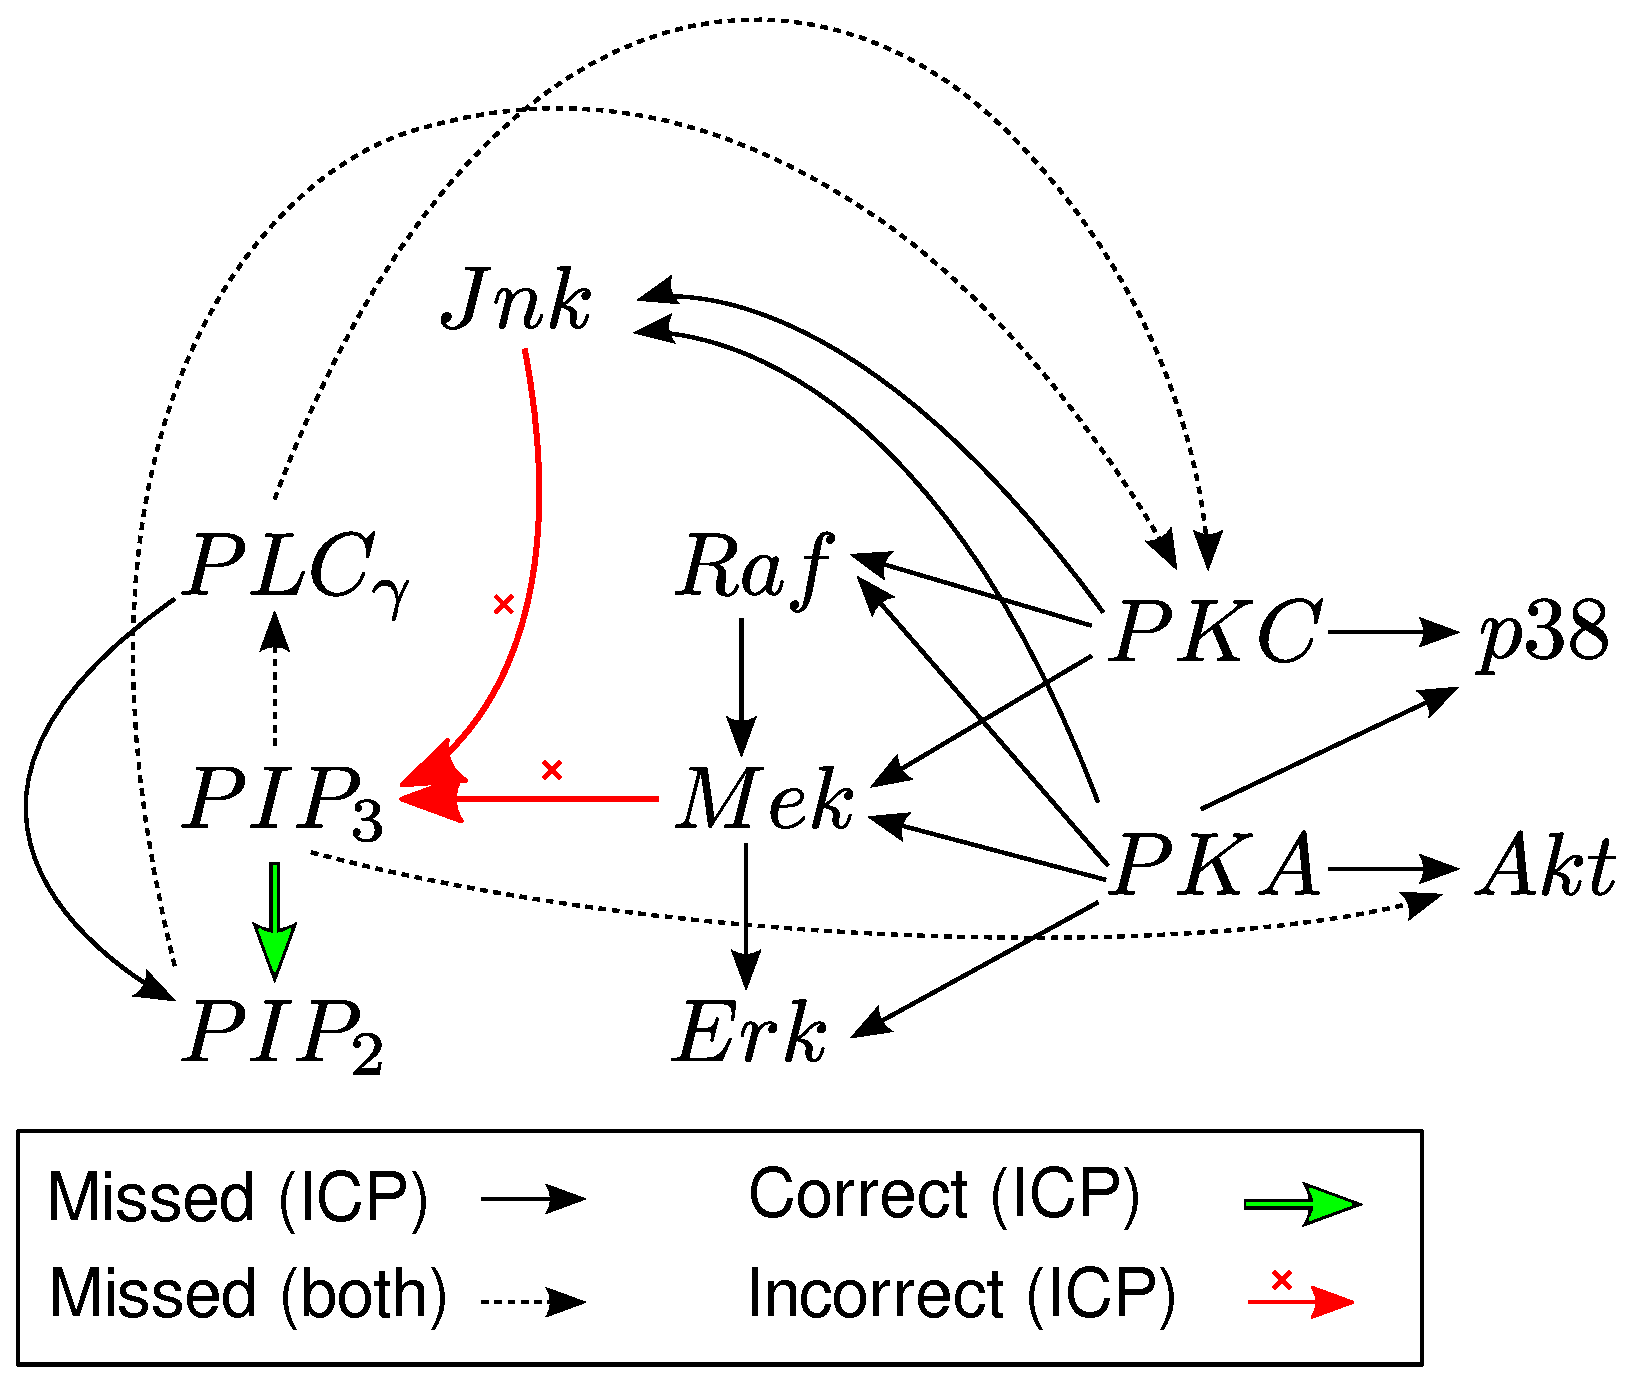
\includegraphics[scale = 0.3]{drawing2legend.eps}
\caption{Application of ICP procedure to recover protein signaling network.
ICP discovered one arrow correctly and two incorrent arrows. No other
discoveries were reported.}
\label{fig:sachs}
\end{figure}

The overly-restrictive linear model could be the reason for the poor
performance of ICP on this dataset. The authors take this as a
robustness property, but it also means ICP is very sensitive to
modeling assumption. A small departure from the linear
model can result in no causal discovery. We did not find in the paper a
summary of the robustness of ICP, so we tried our best to outline in
Table \ref{tab:icp} the behavior of linear ICP when some of its
assumptions are not met. [[Charles, can you explain the
{\color{red} behaviors} in the table?]] The authors are welcomed to
comment on the table and point out any inconsistency if there is any.

\begin{table}[h]
\centering
  \begin{tabular}{|c|c|}
    \hline
    \textbf{Issues} & \textbf{ICP's behavior} \\
    \hline
    Intervene on $Y$ (or a missing cause) &
    $\underset{\emptyset}{\bigcap}$ \\
    \hline
    Non-linear, non-additive, and/or heteroskedastic &
    $\underset{\emptyset}{\bigcap}$ \\
    \hline
    Not enough interventions &
    \textcolor{red}{False causal positives} \\
    \hline
    Small sample size &
    $\emptyset$ \\
    \hline
    Left out a confounder & $\underset{\emptyset}{\bigcap}$ \\
    \hline
    Left out an unconfounding predictor & okay  \\
    \hline
    Misspecified noise model$^2$ & \textcolor{red}{False positives}\\\hline
  \end{tabular}
\caption{Robustness properties of ICP procedure.  Under certain types
  of model misspecifiaction, ICP will return a ``model reject'',
  denoted by $\cap_{\emptyset}$ (i.e.\ all subsets including the empty
  set are not invariant), rather than produce false positives.}
\label{tab:icp}
\end{table}

\bibliographystyle{plainnat}
\bibliography{ref}


\end{document}
